\chapter{Numerical study of impact of vegetation on urban microclimate}
\label{ch:impactofvegetation}
\def\figdir{chapters/ch08_numericalstudy/figures}	
%\begin{quote} 
%	\begin{flushright}
%		\textit{The true logic of this world is in the\\ 
%			calculus of probabilities.}
%		
%		--- ~ James C. Maxwell
%	\end{flushright}
%\end{quote}

\section{Introduction}

In this chapter, the fully coupled (integrated) numerical model, described in \cref{ch:numericalmethod}, is used to assess the impact of vegetation on urban microclimate. To accurately assess the impact of vegetation on urban microclimate, we must determine: i) the influence of vegetation on the turbulent air flow, ii) the influence of plant transpiration on hygrothermal conditions, iii) the influence of plant shading on the urban environment, and iv), the net influence of all the parameters on the pedestrian thermal comfort. In this chapter, the influence of vegetation is assess using two different experimental setups: a) the study on the influence of vegetation on microclimate of a urban street canyon, and b) a case study on the influence of vegetation is a realistic city topology in Z\"urich, Switzerland at a location known as Muensterhof (in german: M\"unsterhof). The Muensterhof is a town square within the city of Z\"urich with that currently lacks vegetation. The objective of the study in the urban street canyon is to perform a parameteric study and determine the parameters that play a key role in improving the thermal comfort. Furthermore, the plant transpiration and the influence on the soil moisture is investigated. The objective of the case study in M\"uensterhof is determine the microclimate modification of vegetation in a realistic setting.

\section{Urban street canyon}

A numerical assessment of the impact of vegetation is first performed in urban street-canyon. The study investigates the influence of transpirative and shaded cooling due to vegetation on the pedestrian comfort inside a street canyon. In this study, we investigate the cooling potential of vegetation, such as a row of trees, on the microclimate of a street canyon using a CFD model in OpenFOAM. Prior to this study, the cooling effect of vegetation (Manickathan et al., 2018) and the microclimate of a street canyon (Kubilay et al., 2017) were studied separately. The present study is a continuation of these works towards modeling their interactions. A radiation model is developed to model the short-wave and long-wave radiative heat fluxes between the leaf surface and the surroundings. Using the developed model, it is possible to study the influence of transpirative cooling and shading due to vegetation on pedestrian thermal comfort inside a street canyon. The thermal comfort for pedestrians is evaluated using Universal Thermal Climate Index (UTCI). 

The study shows that both shading and transpiration have a direct positive influence on the temperatures measured in the street canyon. Moreover, the cooling due to shading is seen to be larger than the transpirative cooling, especially under the tree.

\subsection{Simulation setup}

The simulations are performed for a street canyon with a vegetation zone of $2 \times 10 \times 4$ m$^3$, representing a row of trees which are surrounded by two buildings of $10 \times 50 \times 10$ m$^3$ ($x\times y \times z$), as shown in \cref{fig:domain_new5}. The numerical domain size is $230\times 250 \times 60$ m$^3$  ($x\times y \times z$), where the inlet, outlet, top, and side walls are positioned $5 H$, $5 H$, $15 H$, and $10 H$, respectively, based on CFD best practices \citep{Blocken2015, Franke2007, Tominaga2008}. The numerical domain is discretized into $\num{1178080}$ hexahedral cells with minimum cell size of $\num{1e-3}$ m$^{-3}$ near the building walls (see \cref{fig:mesh_resolution}) and are determined following a grid-refinement study. The vegetation zone has a foliage height of $4$ m (with $z_{\textit{min}}= 4$ m), leaf area density $a= 10$ m$^2$\,m$^{-3}$, leaf drag coefficient $c_d=0.2$ and leaf size $l=0.1$ m. The building are oriented perpendicular the with direction. The meteorological data are based on a typical meteorological year and the total solar radiation intensity is for a clear sky on the 21$^{\mathrm{st}}$ of June in the city of Z\"urich, Switzerland used in the study of \cite{Kubilay2018}. The wind speed at the building height is $U_{\textit{ref}}=5$ m\,s$^{-1}$ where turbulence kinetic energy $k$ and turbulence dissipation rate $\varepsilon$ are determined using \cref{eq:ableq} \citep{Richards1993} with $u_*/U = 0.072$ and $z_0 = 0.03$ m. Standard wall functions are employed for the wall boundary and a constant static pressure of $p=0$ Pa at the outlet boundary. The inlet, top and side wall are prescribed with the ambient temperature varies between 11$^{\circ}C$ and 19 $^{\circ}C$ with solar noon at $13:28$ and the relative humidity varies between 62\% and 86\% $RH$ as shown in \cref{fig:meteobc}. 

	\begin{figure}[t]
	\centering
	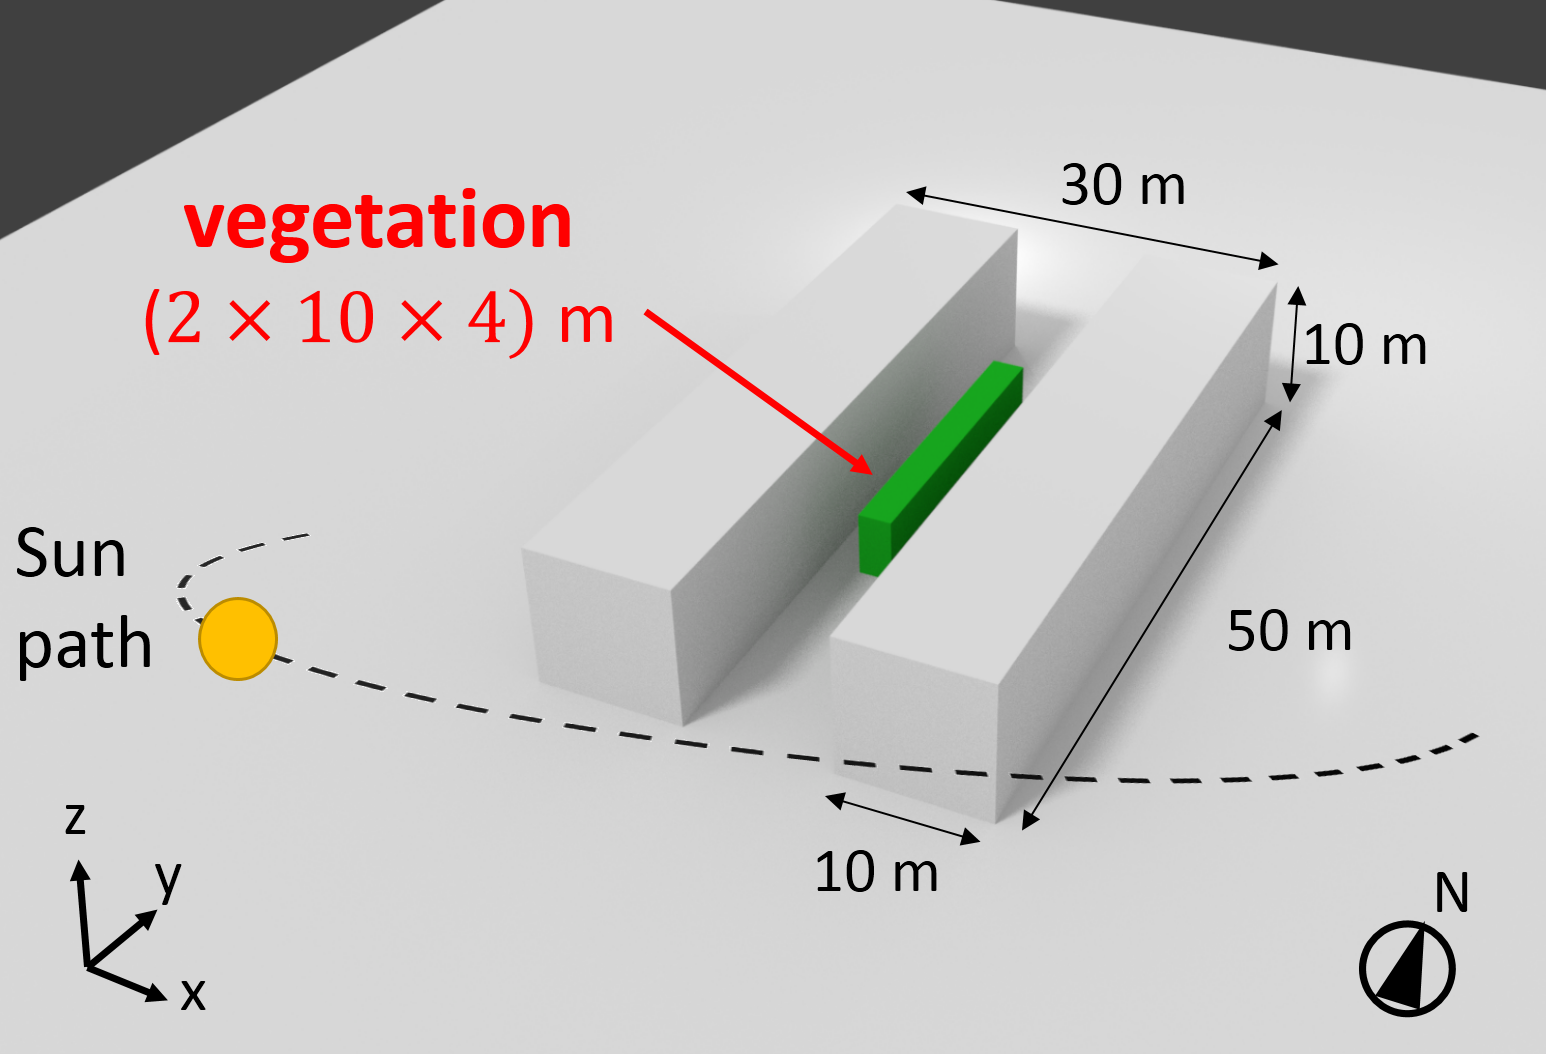
\includegraphics[width=0.8\textwidth]{\figdir/domain_new5.png}
	%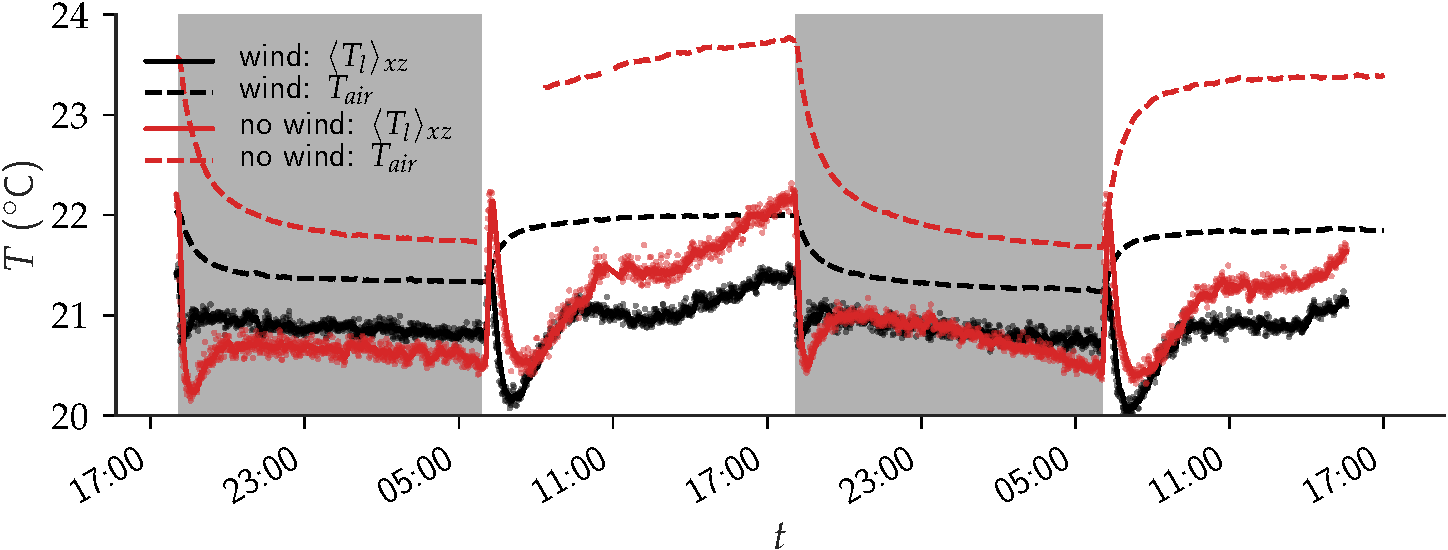
\includegraphics[width=\textwidth]{\figdir/Tinfrared_vs_air_updated-crop.pdf}
	\caption{The simulation setup of a street canyon composed of two buildings measuring $10 \times 50 \times 10$ m$^3$ ($x\times y \times z$) with vegetation band of size $2 \times 10 \times 4$ m$^3$ in the center. The setup is based on the study of Kubilay et al. (2017) with wind.}
	\label{fig:domain_new5}
	\end{figure}


\begin{figure}[p]
	\centering
	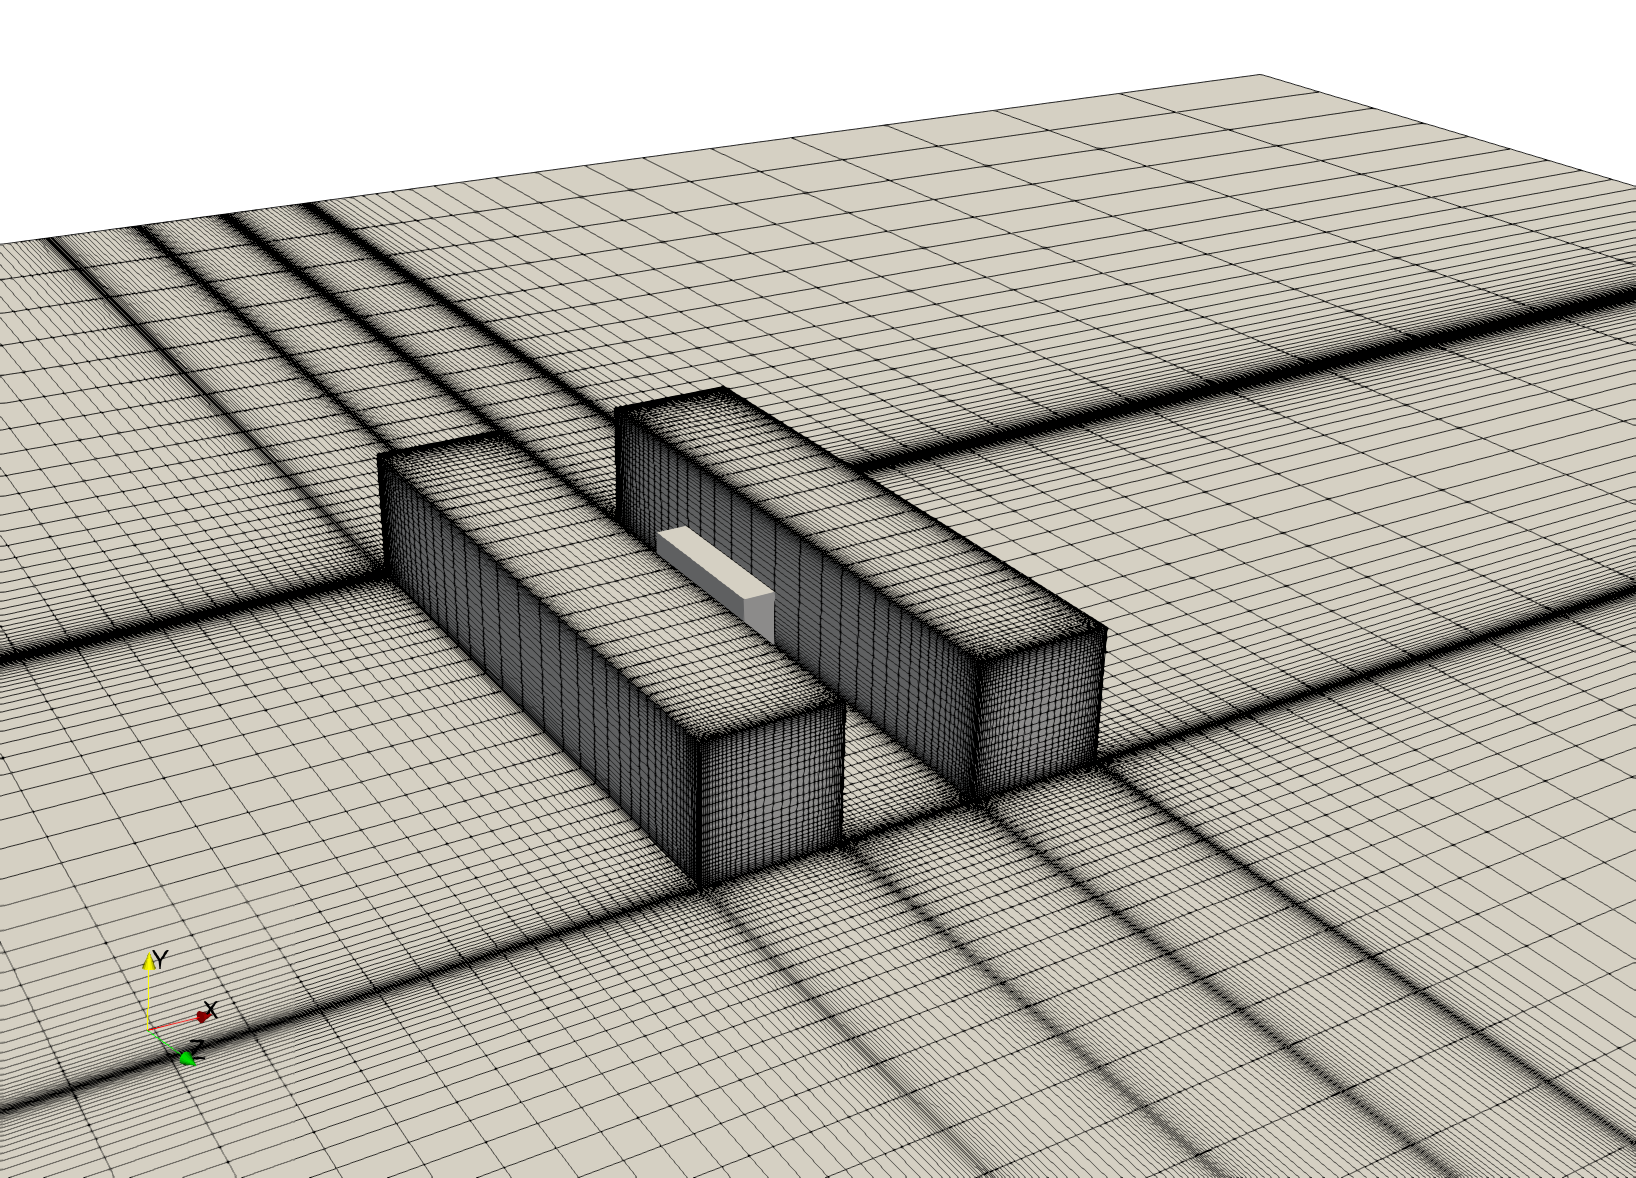
\includegraphics[width=0.6\textwidth]{\figdir/mesh_resolution.png}
	%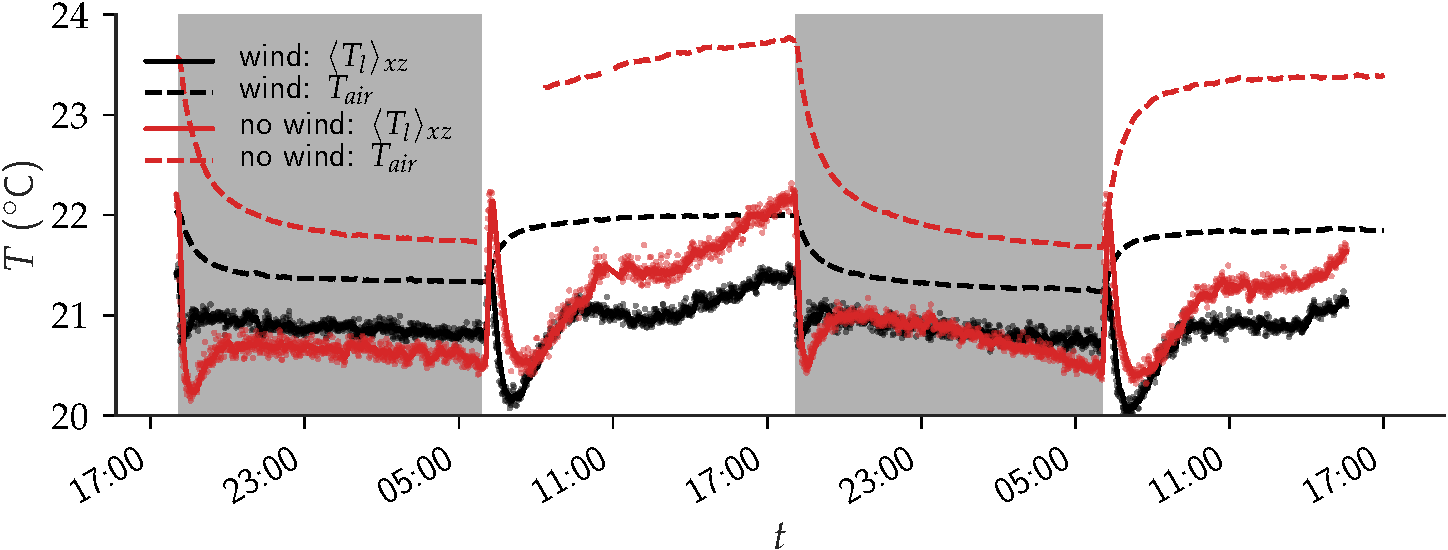
\includegraphics[width=\textwidth]{\figdir/Tinfrared_vs_air_updated-crop.pdf}
	\caption{Simulation domain showing the surface layer mesh refined closed to the building walls. The numerical domain is discretized into $\num{1178080}$ hexahedral cells with minimum cell size of $\num{1e-3}$ m$^{-3}$ at the building corner. The mesh is based on the study of \cite{Kubilay2018}.}
	\label{fig:mesh_resolution}
\end{figure}

\begin{figure}[p]
	\centering
	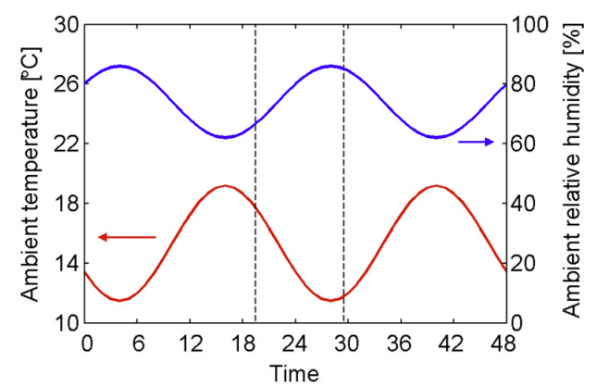
\includegraphics[width=0.8\textwidth]{\figdir/meteobc.png}
	%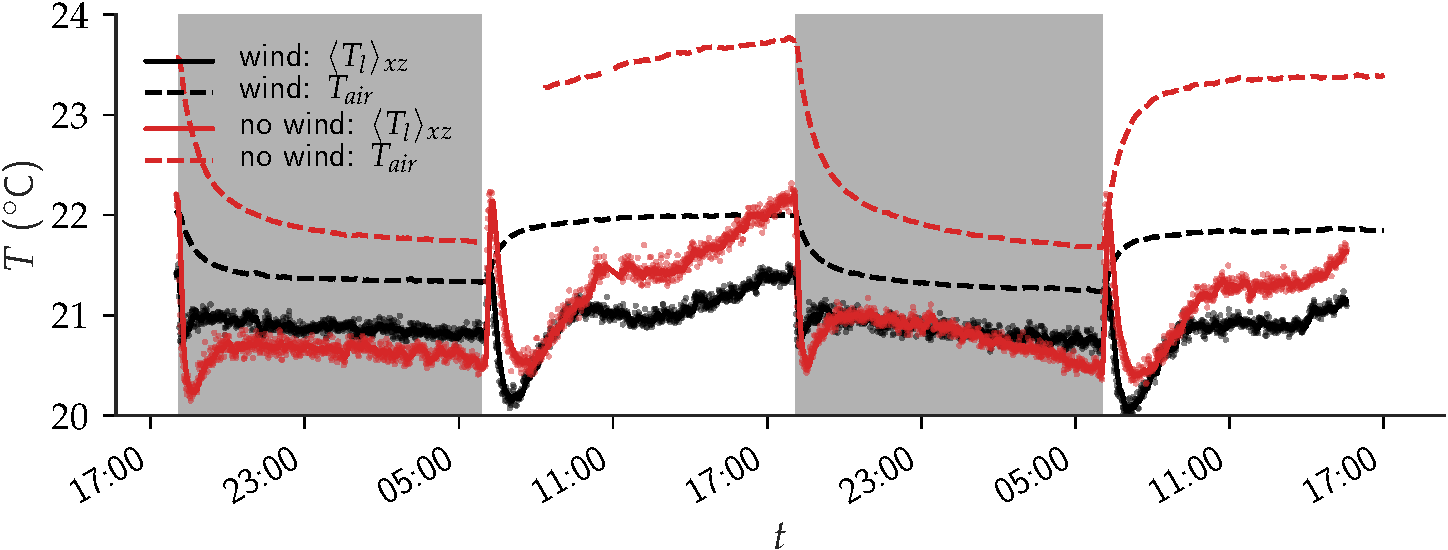
\includegraphics[width=\textwidth]{\figdir/Tinfrared_vs_air_updated-crop.pdf}
	\caption{Diurnal ambient temperature $T$ ($^{\circ}C$) and relative humidity $RH$ (\%) profile obtained from \cite{Kubilay2018}. The meteorological data are based on a typical meteorological year and the total solar radiation intensity is for a clear sky on the 21$^{\mathrm{st}}$ of June in the city of Z\"urich, Switzerland. }
	\label{fig:meteobc}
\end{figure}

\begin{figure}[p]
	\centering
	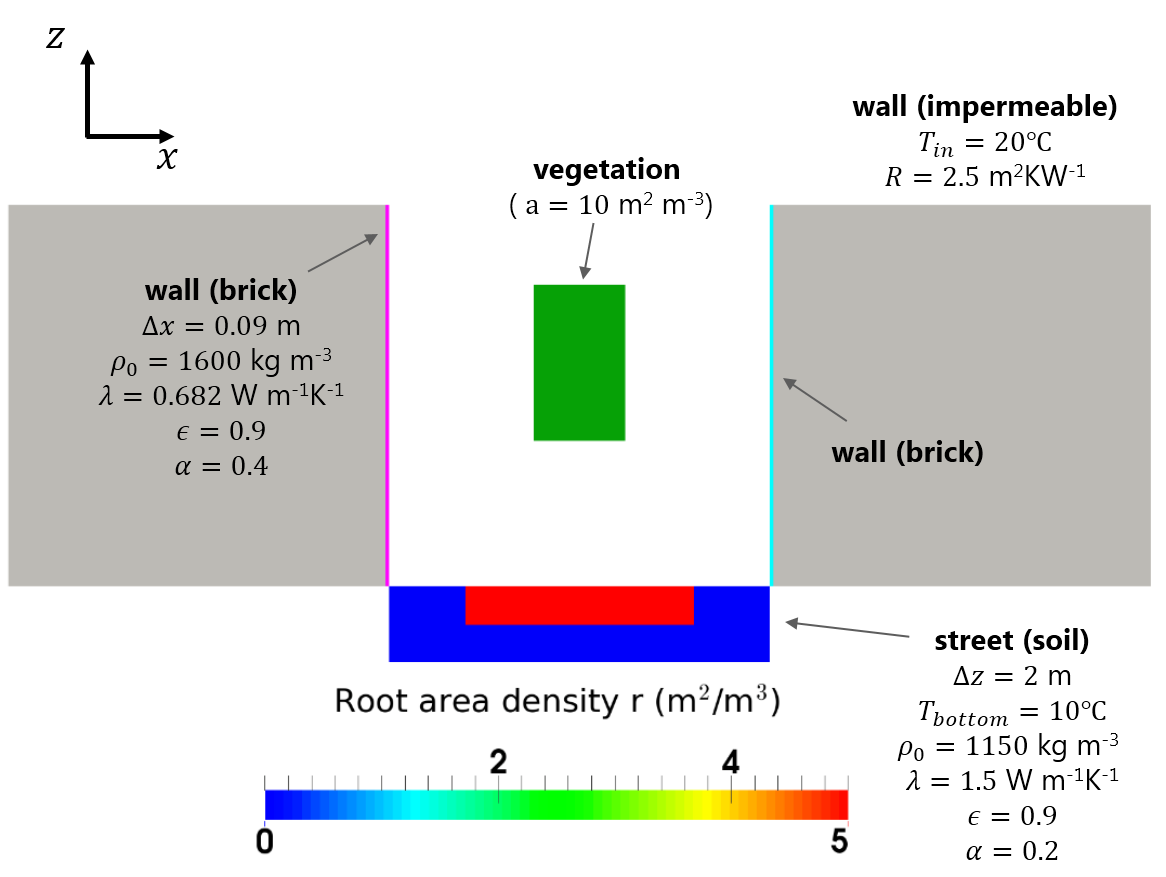
\includegraphics[width=\textwidth]{\figdir/soliddomain_v2.png}
	%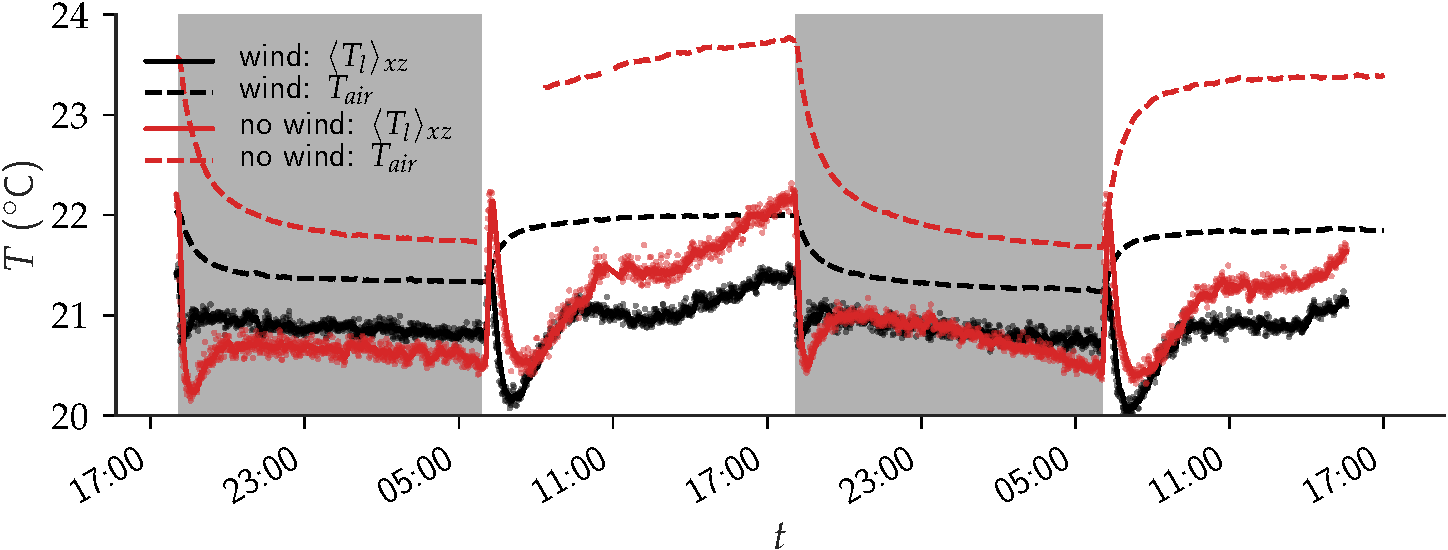
\includegraphics[width=\textwidth]{\figdir/Tinfrared_vs_air_updated-crop.pdf}
	\caption{Description of the solid domain consisting of two impervious buildings of size $10 \times 50 \times 10$ m$^3$ ($x\times y \times z$) each with a brick layer of $0.09$ m inside the street-canyon and a soil region at the street with vegetation roots. The temperature $T_{\textit{in}}$, thermal resistance $R$, the density $\rho_0$, thermal conductivity $\lambda$, emissivity $\epsilon$, albedo $\alpha$, leaf area density $a$ and root area density $r$ and also provided. }
	\label{fig:soliddomain}
\end{figure}


The diurnal variation of the microclimate is modeled using the approach discussed in \cref{ch:numericalmethod}, where the air domain, solid domains (i.e., leeward and windward building wall made of brick and street region where the roots are present is made of soil with equal composition of sand, silt, and clay). \cref{fig:soliddomain} shows the setup of the solid domain, i.e., $x-z$ plane at $y=125$ m ($y$ center of the street-canyon). 


\subsection{Results and Discussion}

The influence of vegetation on the microclimate of the street canyon (depicted in Fig.1) is studied using the developed numerical model. The natural cooling provided by the row of trees is determined by comparing the setup with and without vegetation, “V” and “NV”, respectively. Fig. 2 shows the change in air temperature, $T_v-T_nv$ at noon (12 pm), when the sun is directly above the street canyon. The vegetated region is indicated by the dashed outline. From the figure, two distinct regions of cool zones can be identified. The first region is at the vicinity of the vegetation with a temperature change of around -2 . This cool zone results from the transpirative cooling effect of vegetation. 

%	\begin{figure}[t]
%	\centering
%	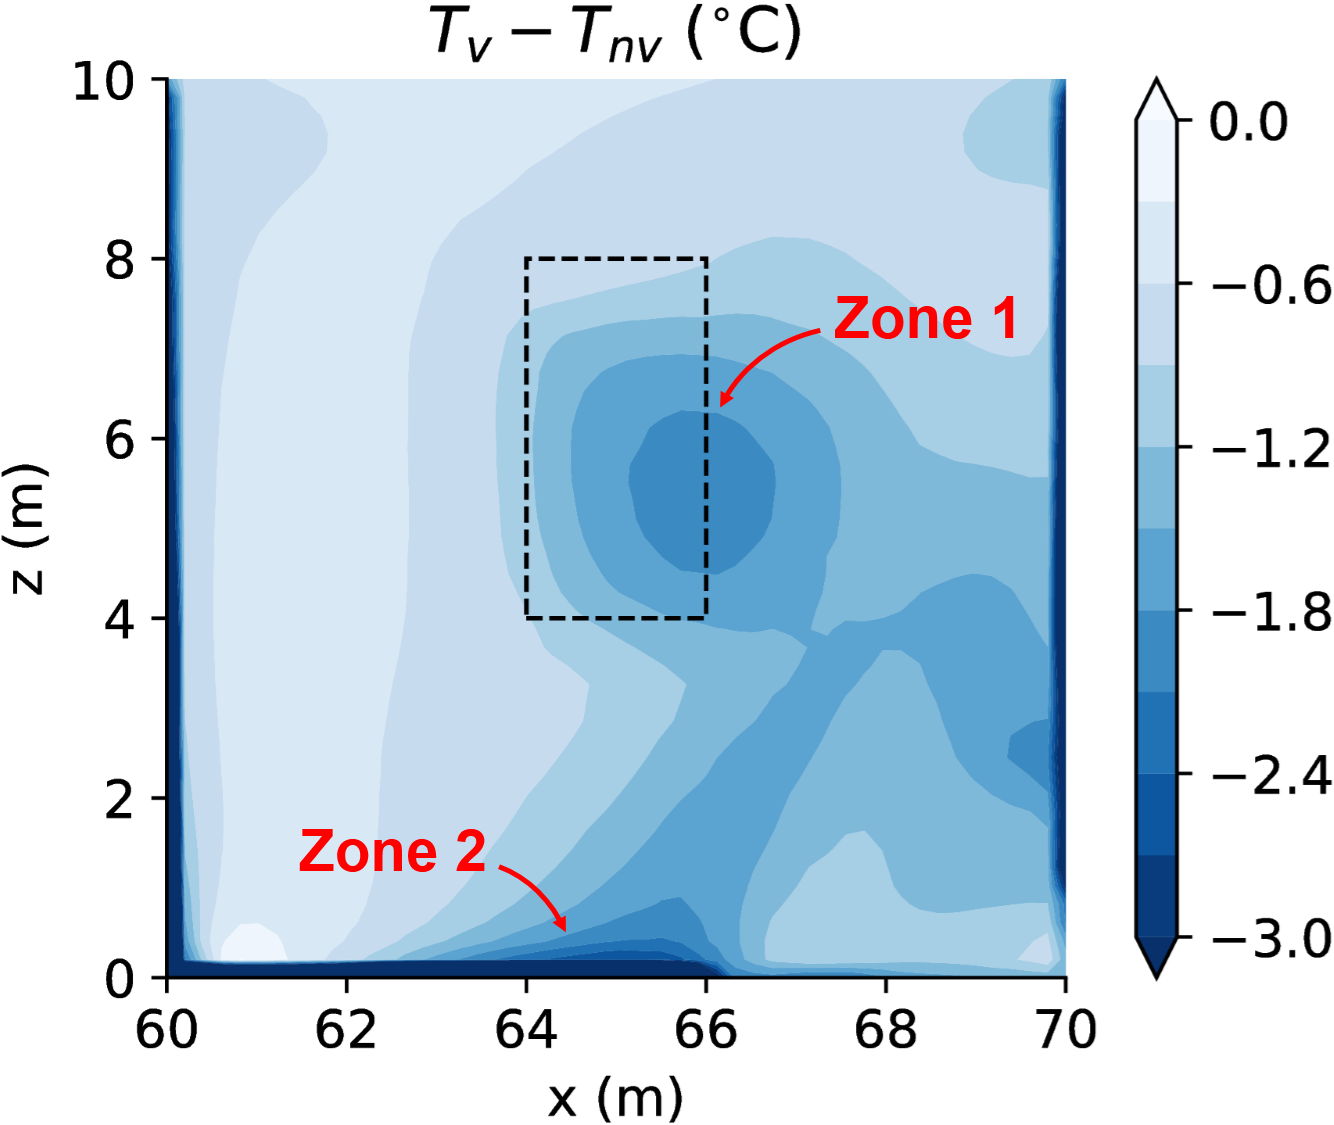
\includegraphics[width=0.6\textwidth]{\figdir/DT_field_v2.png}
%	%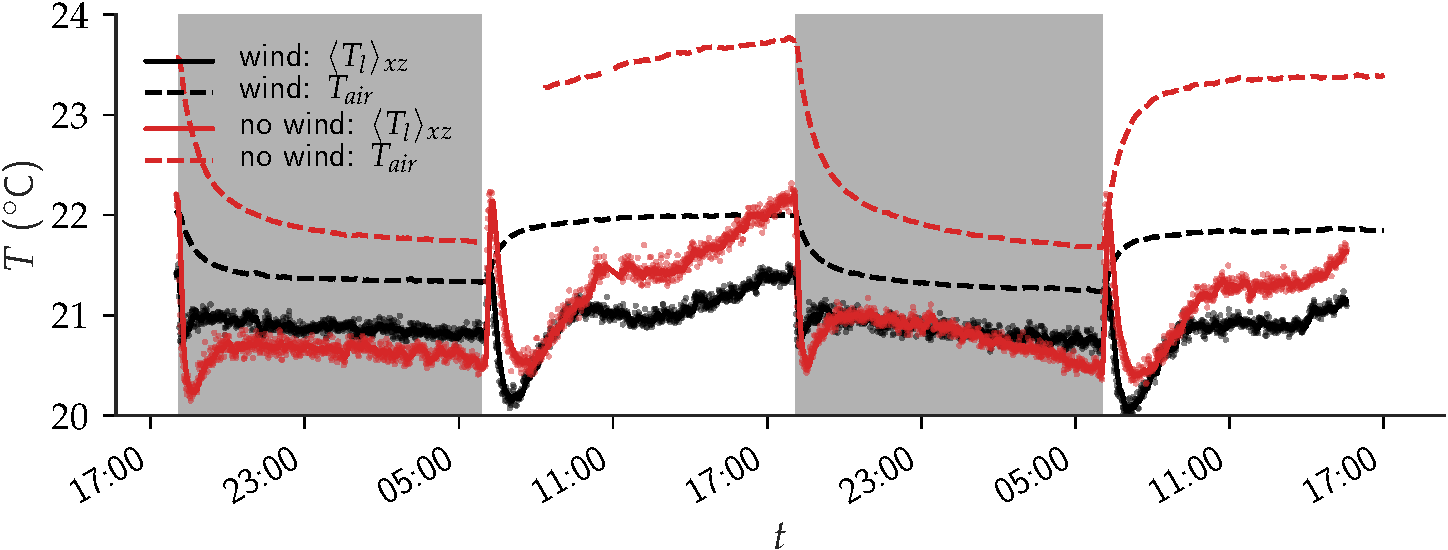
\includegraphics[width=\textwidth]{\figdir/Tinfrared_vs_air_updated-crop.pdf}
%	\caption{Temperature drop, $Tv - Tnv$ (℃) due to vegetation at noon (12 pm) in the center of the street canyon (at $y= 125$ m). The vegetated zone (i.e., row of trees) is indicated by the black dashed line.}
%	\label{fig:DT_field_v2}
%	\end{figure}

\subsubsection*{Influence of plant transpiration}

\begin{sidewaysfigure}[p]
	\centering
	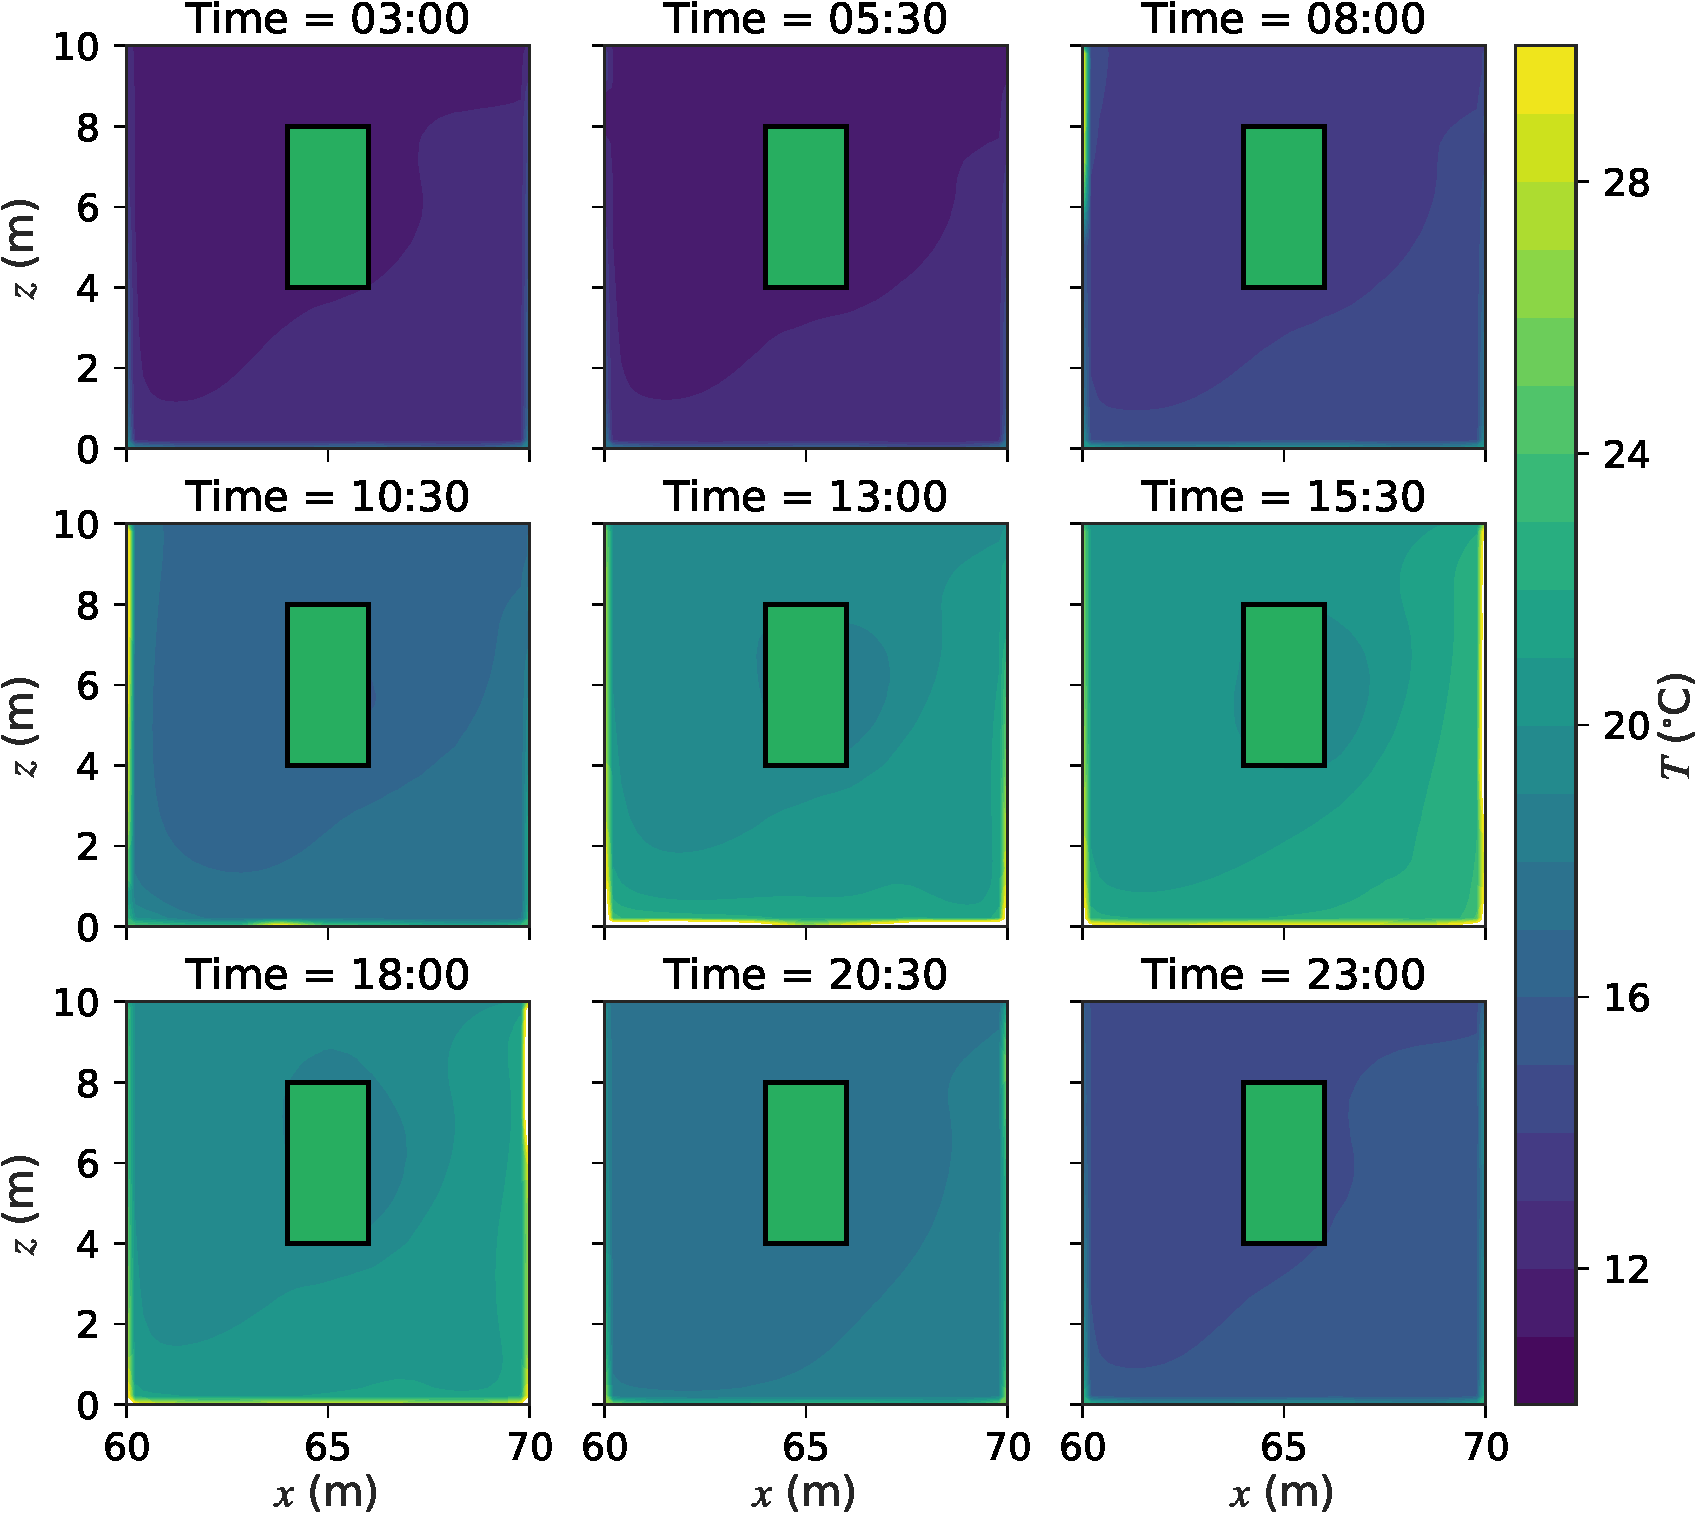
\includegraphics[width=0.9\textwidth]{\figdir/USC_T-crop.pdf}
	\caption{T field}
	\label{fig:USC_T}
\end{sidewaysfigure}



The second zone is the region close to the building wall, where the shadow of the tree was present earlier during the day. This cooling region, resulting from tree shading, is seen to be more effective than the transpirative cooling region, showing a temperature drop of more than -3. Furthermore, at the current location of the shadow, the cooling air is seen to be convected away from the wall, and interacts with the cool zone. This indicates that, in addition to transpirative cooling, the tree-shade cooling plays a vital role in improving the microclimate. It is also evident that, as a result of the combined influence of transpirative and tree-shade cooling, the overall surface temperature of the street canyon is lower.

To quantify and distinguish the natural cooling associated with transpirative cooling and the natural cooling associated with tree-shade cooling, two simulation cases are compared: transpiration and shaded case (T+S) and shade only case (S). Fig. 3 compares the diurnal variation of the temperature drop, $T_v-T_nv$, for these two configurations, for a single measurement point below the row of trees at x= 65 m, y= 125 m and height of z= 2 m. The peak reduction in air temperature below the tree is seen to occur at noon, when the point is under the shadow. The configuration “S”, with only shadow, shows a peak air temperature drop of around -1.0 ℃ whereas with transpiration (T+S), an additional temperature drop of -0.2 is found. Therefore, the tree-shade cooling is dominant here. Furthermore, studying the diurnal variation, it is evident that the cooling effect of vegetation is also present during the night time, even after transpiration and tree shade are no longer present, with a temperature drop of around -0.4. This indicates that a reduction in the heat storage inside the buildings has a prolonged benefit to the urban climate.


\subsubsection*{Influence of shading}

\begin{sidewaysfigure}[p]
	\centering
	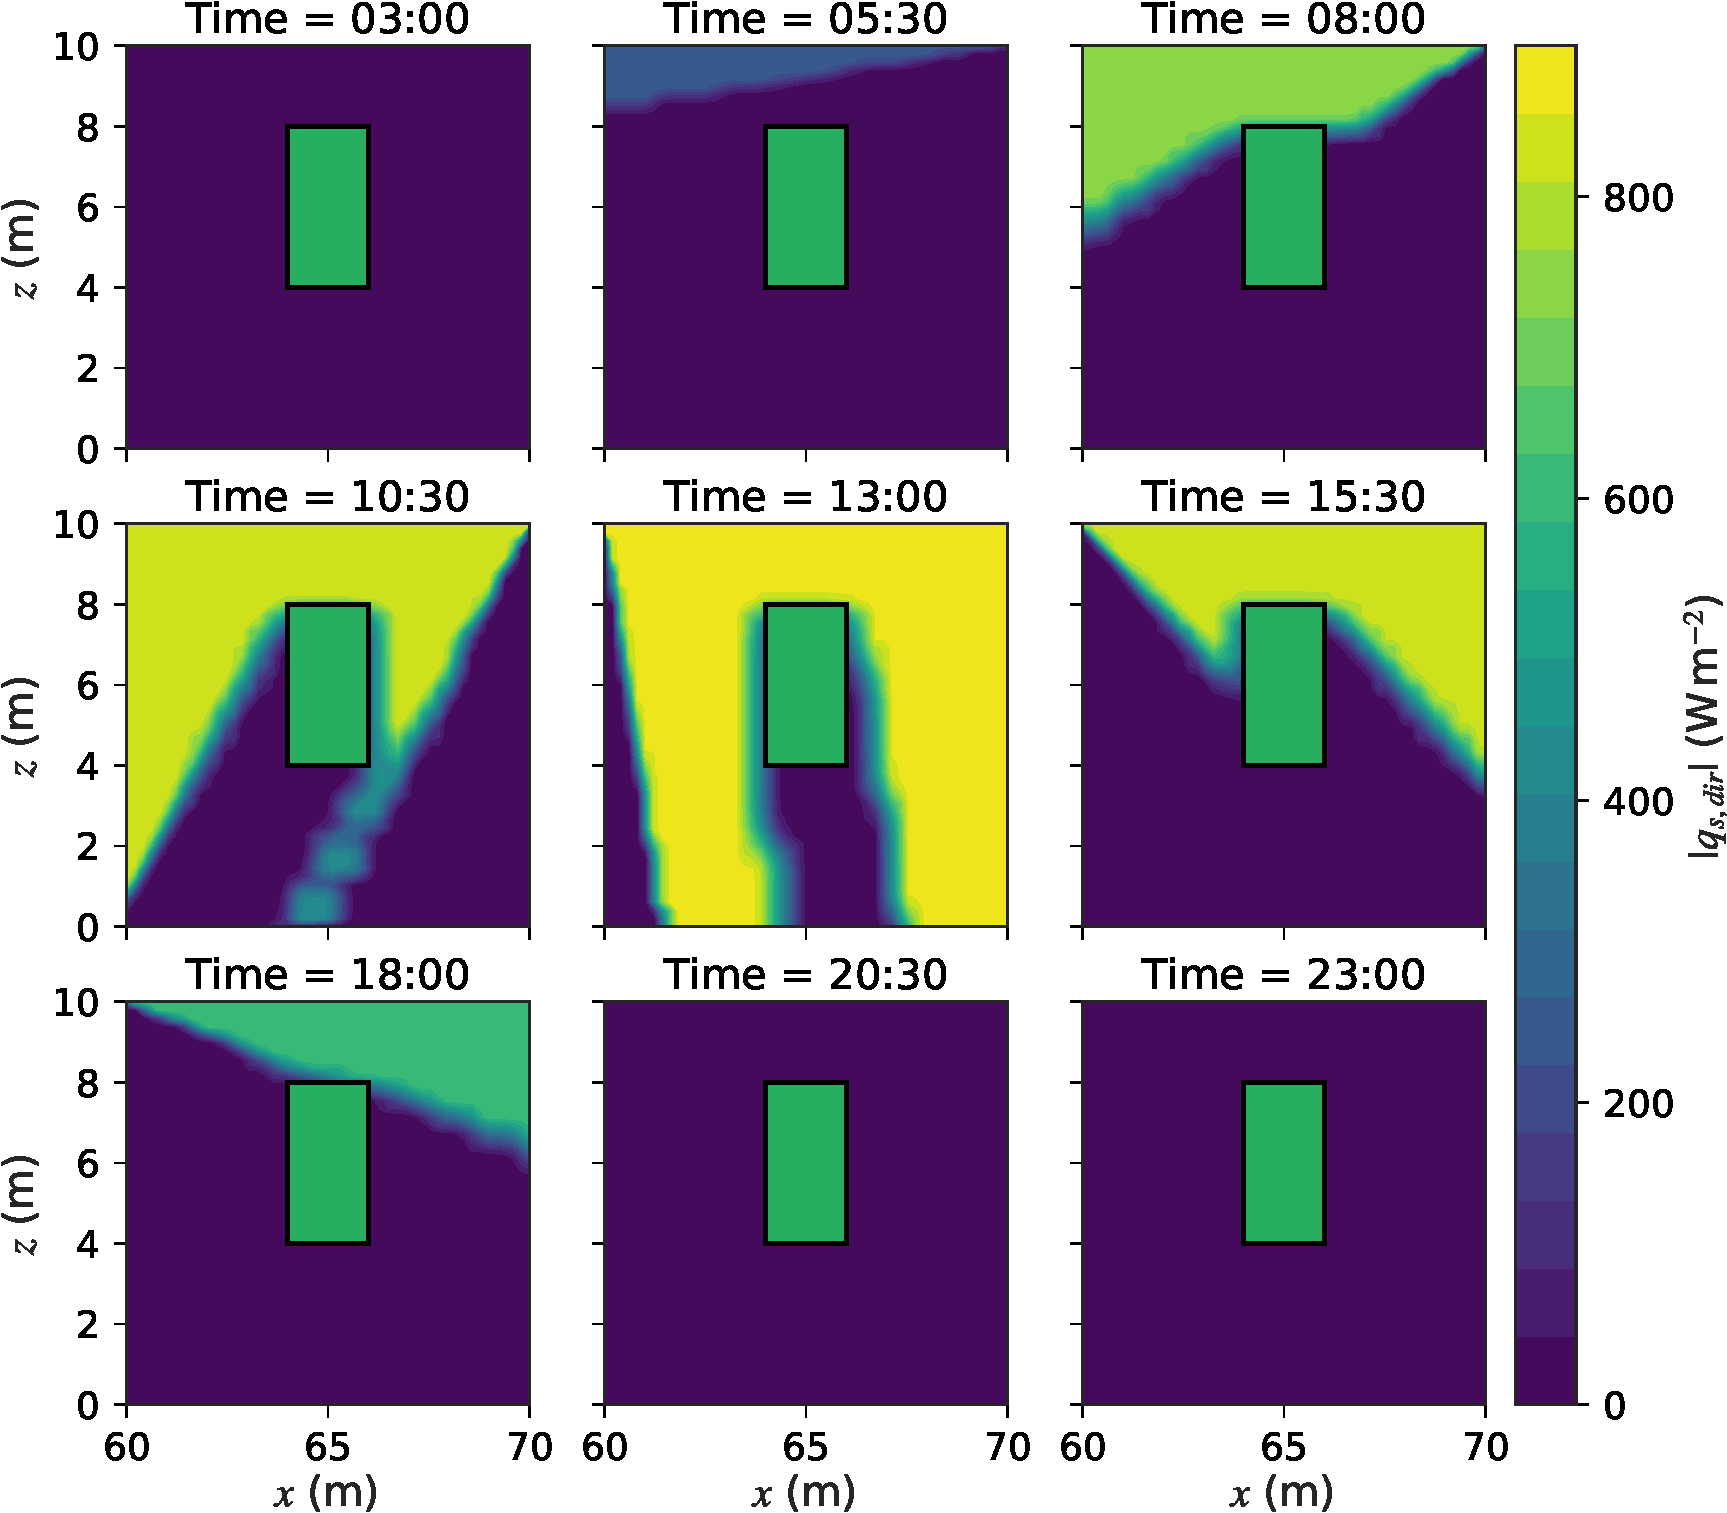
\includegraphics[width=0.9\textwidth]{\figdir/USC_qsdir-crop.pdf}
	\caption{qsdir profile}
	\label{fig:USC_qrdir}
\end{sidewaysfigure}

\begin{sidewaysfigure}[p]
	\centering
	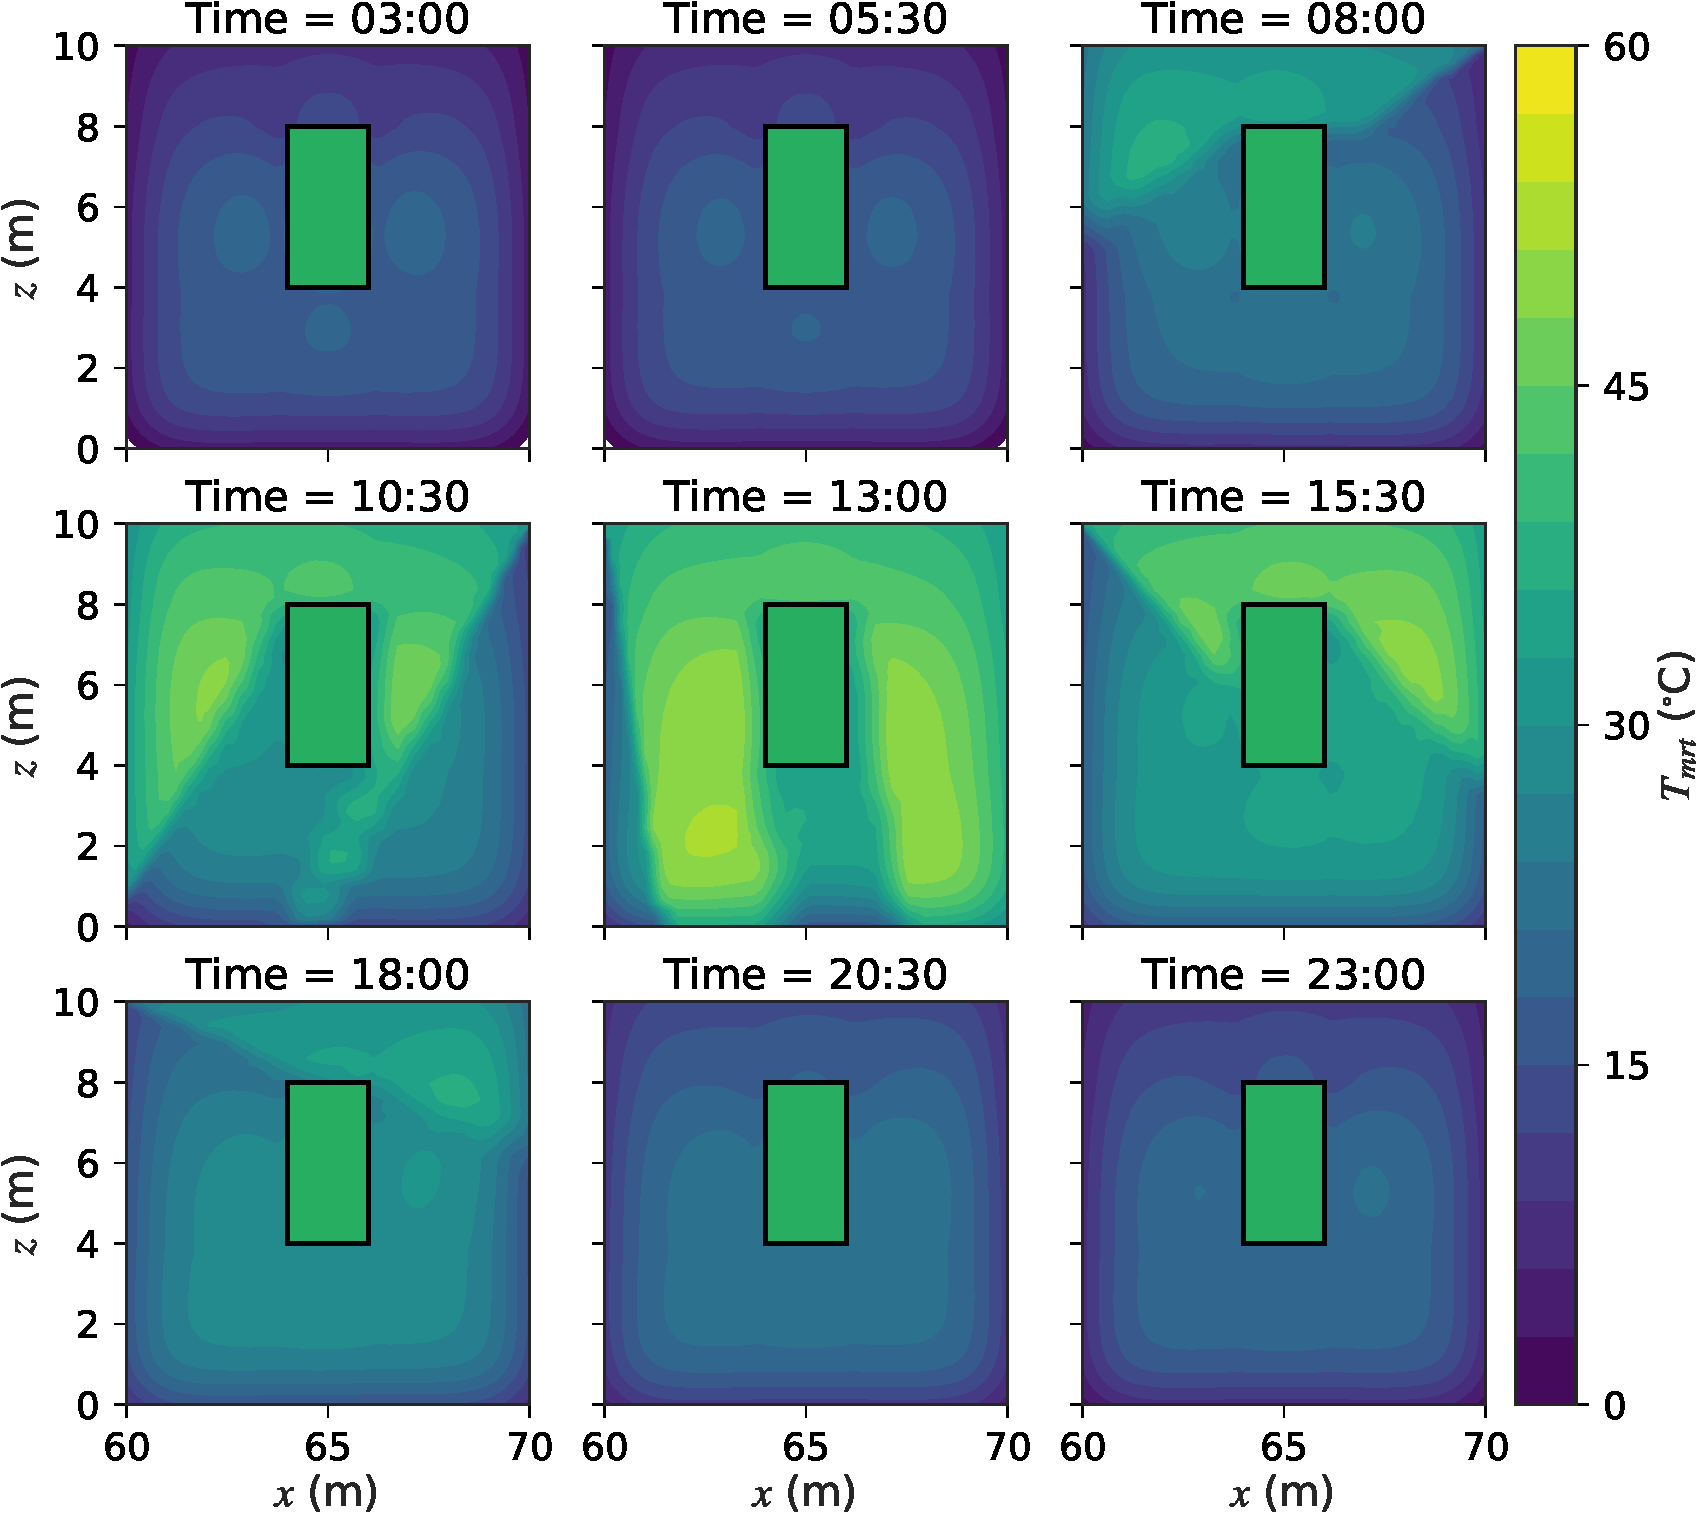
\includegraphics[width=0.9\textwidth]{\figdir/USC_Tmrt-crop.pdf}
	\caption{UTCI profile}
	\label{fig:USC_UTCI}
\end{sidewaysfigure}


\begin{figure}[t]
	\centering
	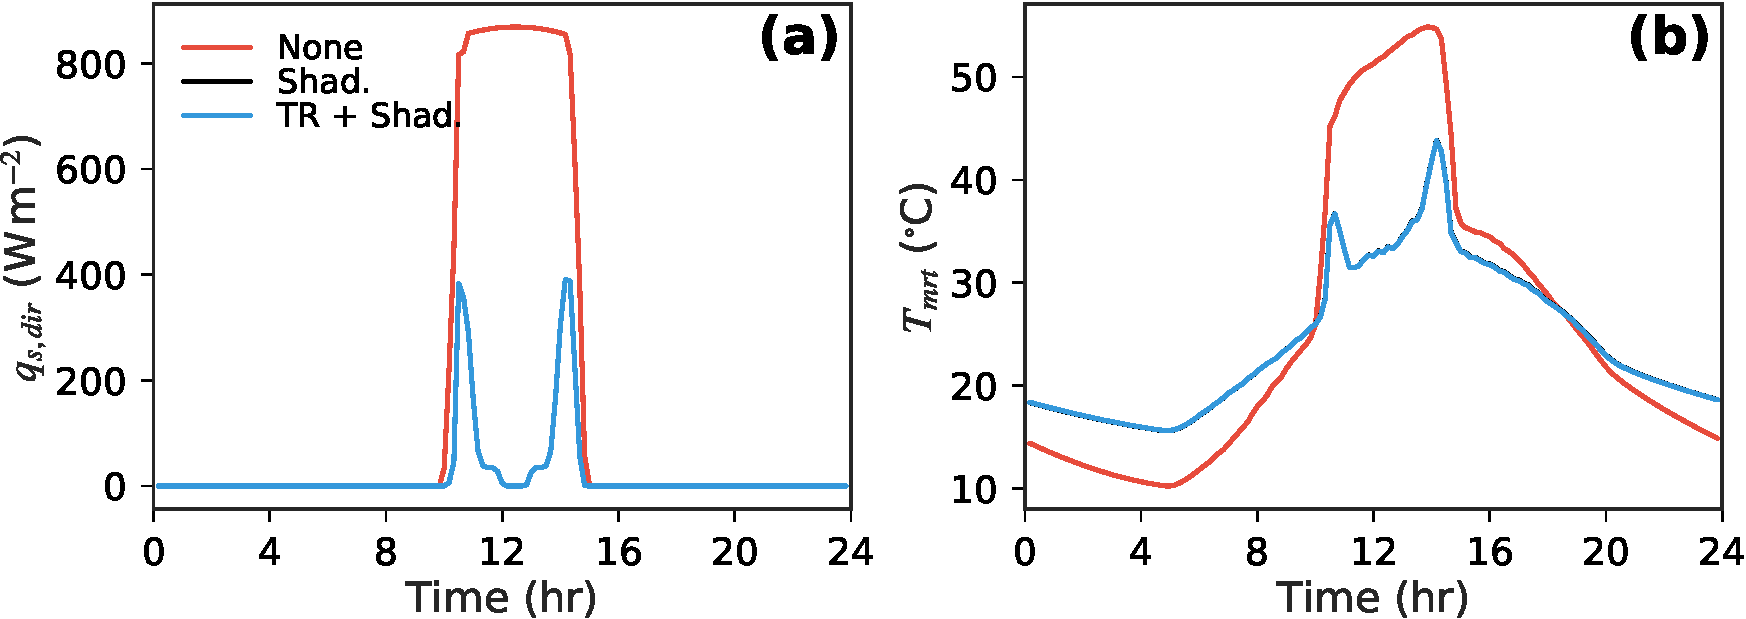
\includegraphics[width=\textwidth]{\figdir/profile_qsdir_Tmrt-crop.pdf}
	\caption{profile qsdir Tmrt}
	\label{fig:profile_qsdir_Tmrt}
\end{figure}

\subsubsection*{Impact of thermal comfort}

\begin{sidewaysfigure}[p]
	\centering
	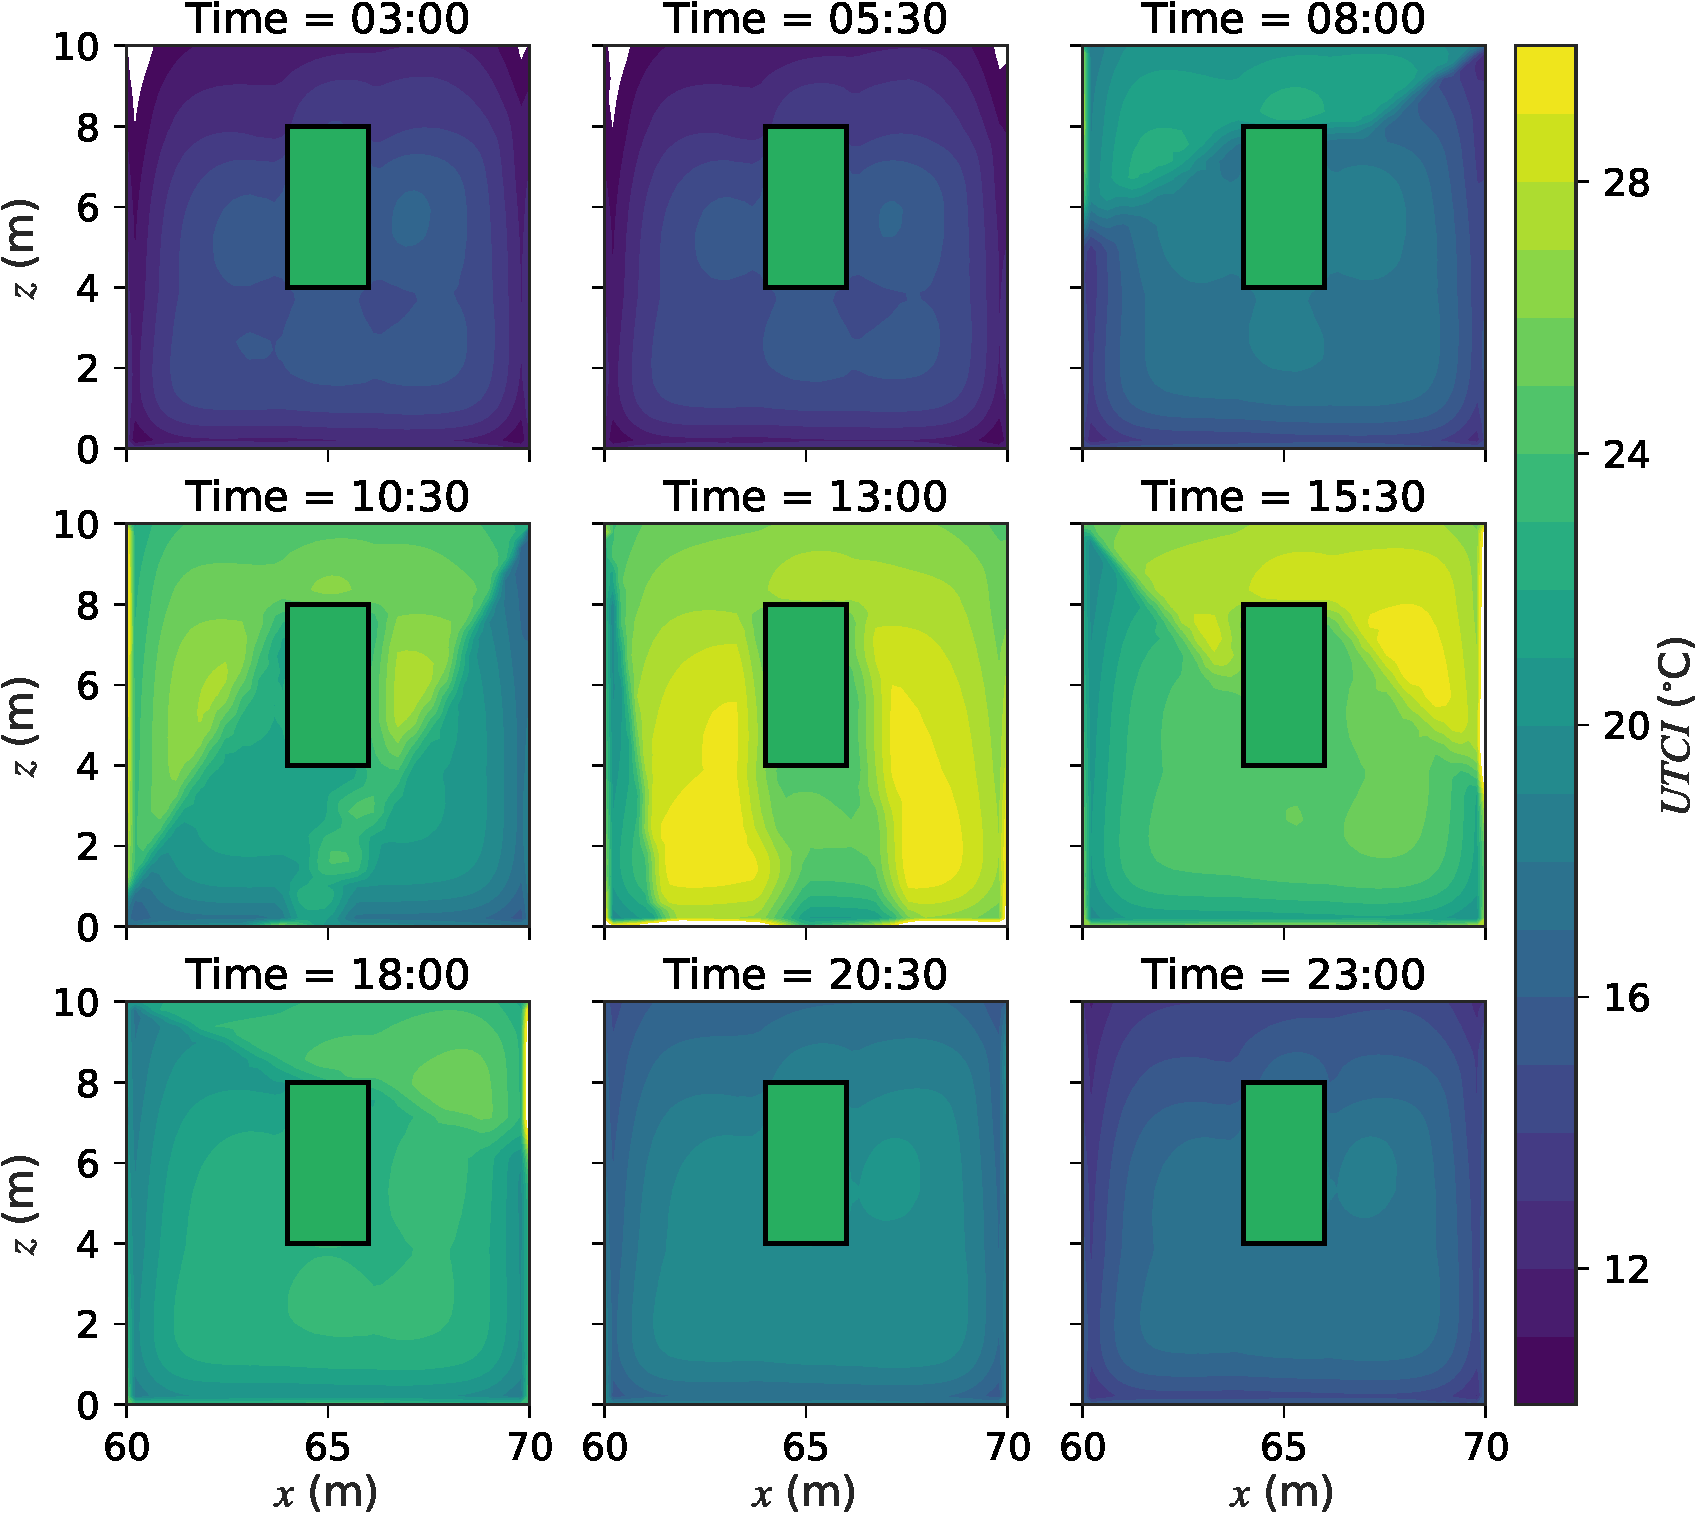
\includegraphics[width=0.9\textwidth]{\figdir/USC_UTCI-crop.pdf}
	\caption{UTCI profile}
	\label{fig:USC_Tmrt}
\end{sidewaysfigure}


\begin{figure}[t]
	\centering
	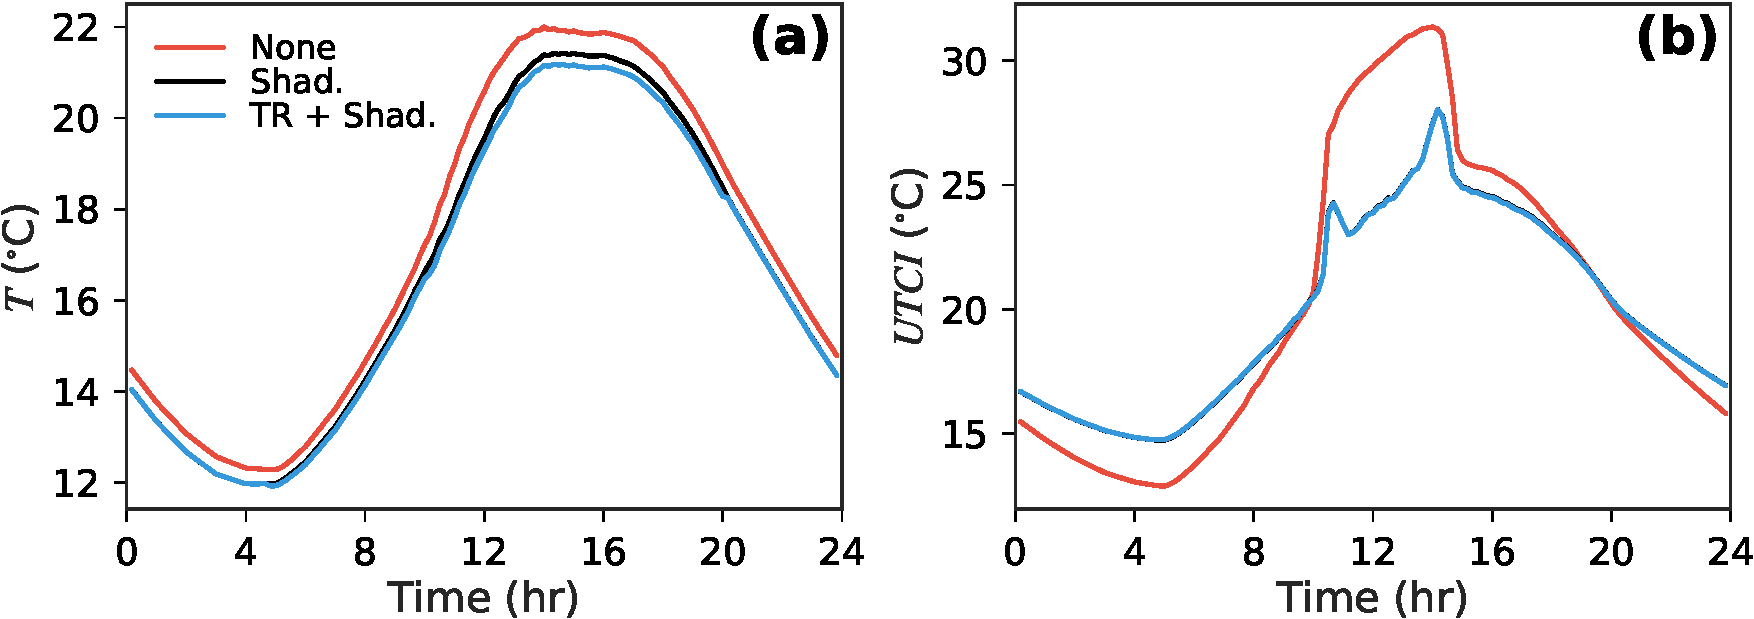
\includegraphics[width=\textwidth]{\figdir/profile_T_UTCI-crop.pdf}
	\caption{profile T UTCI}
	\label{fig:profile_T_UTCI}
\end{figure}


The influence of vegetation on pedestrian comfort is determined by evaluating the Universal Thermal Climate Index (UTCI) (℃) (Fiala et al., 2001; Manickathan et al., 2018). We position a pedestrian under the tree, Fig. 4 shows the diurnal variation of the UTCI for three different cases: setup without vegetation (no veg), setup with only shading vegetation (S) and setup with transpiring and shading vegetation (T+S). The calculated UTCI (below the trees at (x,y,z)= (65, 125, 2) m) shows that the comfort perceived by the pedestrian with and without transpiration is identical. The perceived change in comfort is simply due the change in radiative exchanges, influenced by the vegetation. During night time, the UTCI with vegetation is slightly higher which is possibly due to the long-wave radiation emitted from the vegetation. The thermal comfort provided by the vegetation is most significant when the tree intercepts the solar radiation. At noon, when the measured point is in the shadow of the tree, the UTCI is seen to drop by around 7 ℃, indicating the substantial benefit of the shading on the thermal comfort. In contrast, transpirative cooling is seen to negligibly influence the comfort factor for a pedestrian standing near the tree.

The cooling potential of trees in the street canyon is quantified by studying the diurnal variations of air temperature and humidity for three distinctly different configurations: street canyon without tree, street canyon with trees but only providing shading and, finally, street canyon with trees providing both transpirative cooling and cooling due to shading. The configuration of trees that only provide shading in the street canyon is achieved by artificially closing the stomata in the model. Figure 2 shows the diurnal variation of air temperature and humidity ratio below the tree at z=2 m (point at the middle of the street canyon) for these three configurations. The figure shows that, without the trees, the air temperature is quantifiably higher throughout both day and night. However, once the trees are present, both shading and transpiration provide cooling in the street canyon, with an average decrease of 0.5°C in presence of shading and of an additional 0.2°C, when transpiration is added to shading. The cooling due to shading is seen to be higher than the cooling provided from transpiration. The study on the diurnal variation of humidity ratio inside the street canyon, Figure 2b, shows that the humidity in the street canyon is increased when the trees transpire. This could potentially negatively affect the pedestrian comfort below the tree. 

The universal thermal climate index (UTCI) is employed to study the influence of vegetation on pedestrian comfort inside the street canyon. Figure 3 shows UTCI distribution at the vertical centre-plane of the street canyon at four distinct local times: 06:00, 09:00, 12:00 and 15:00. It is apparent that the pedestrian comfort is significantly compromised due to the exposure to solar radiation at noon. However, inside the shaded zone of the trees, the thermal comfort is substantially improved, as indicated by the reduced UTCI values. In contrast, the impact of humidity generated from the trees is not discernible in the UTCI distribution. This means the transpiration of the trees does not negatively affect pedestrian comfort in the case studied, although an increase in relative humidity could reduce the thermal comfort.


\subsubsection*{Influence of water availability}



\begin{figure}[p]
	\centering
	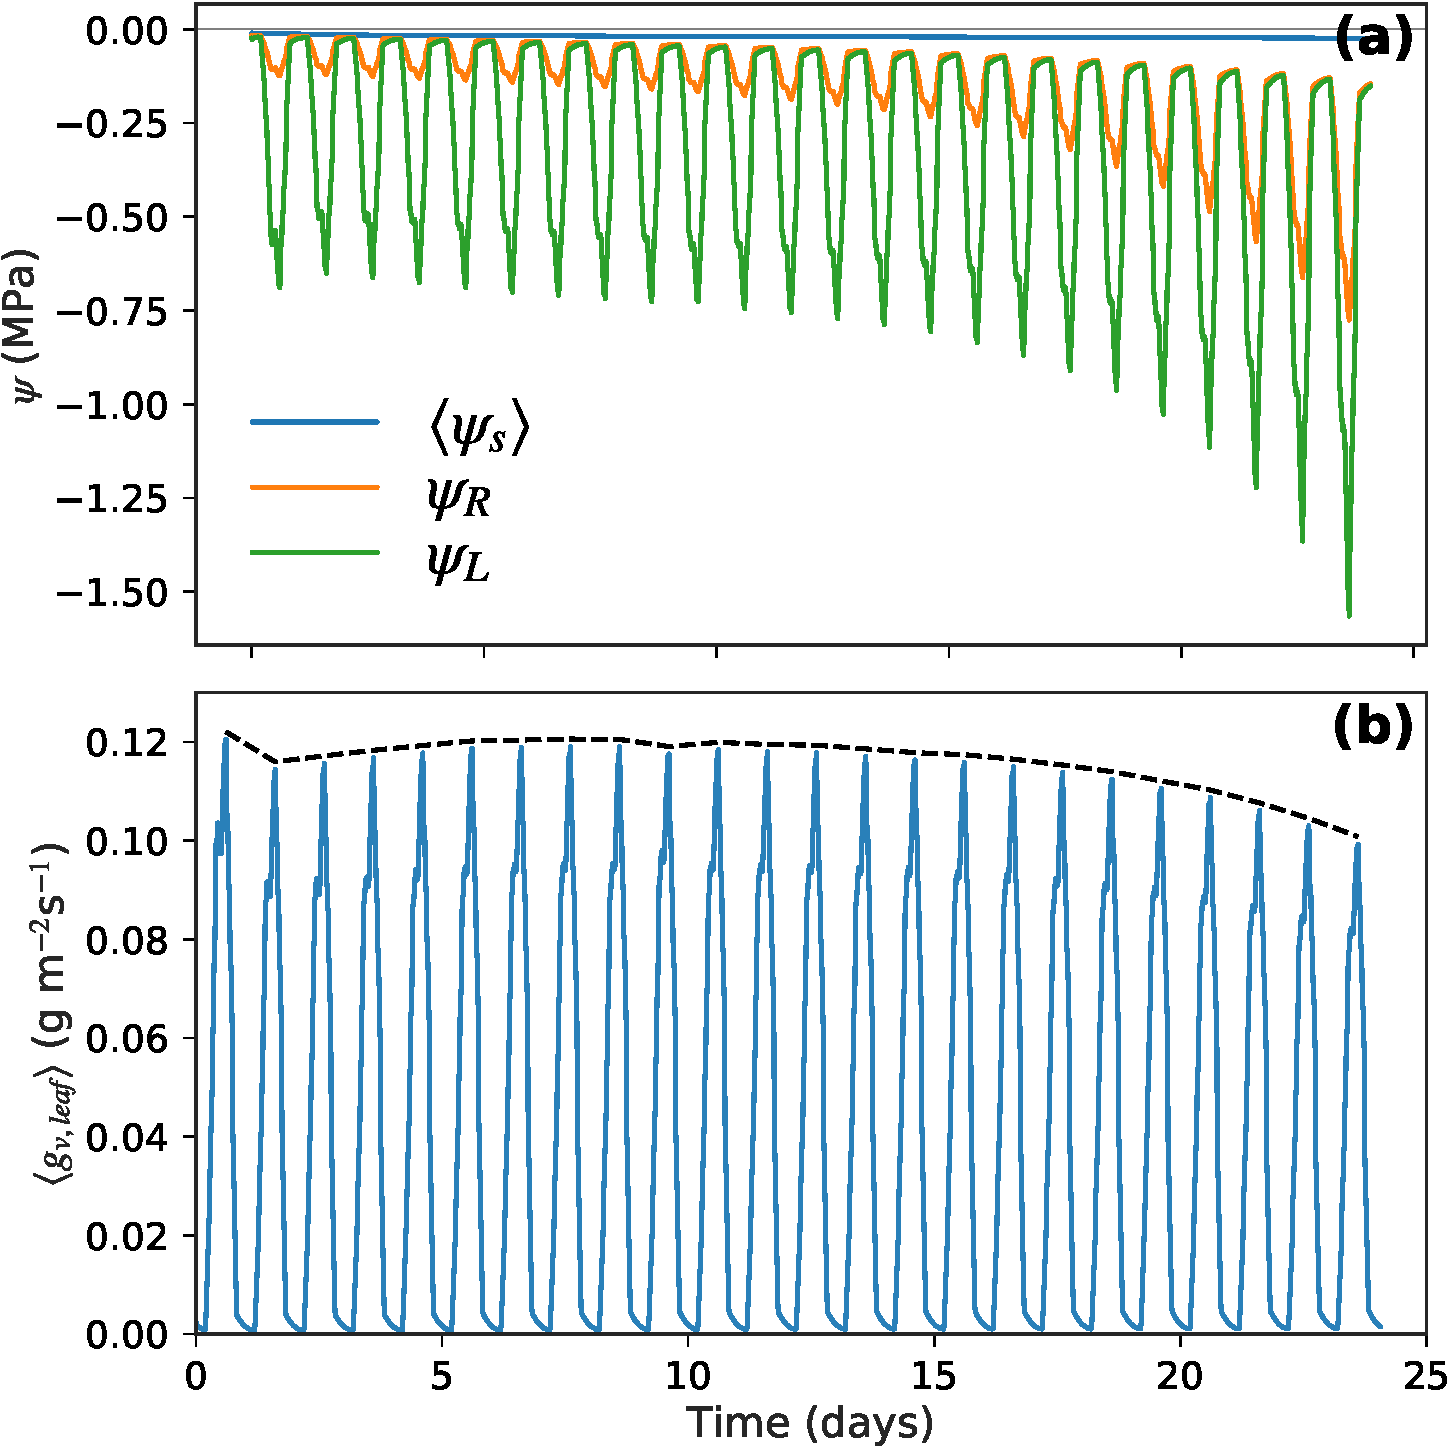
\includegraphics[width=0.8\textwidth]{\figdir/profile_psi_gvleaf-crop.pdf}
	\caption{profile psi gvleaf}
	\label{fig:profile_psi_gvleaf}
\end{figure}


\begin{figure}[p]
	\centering
	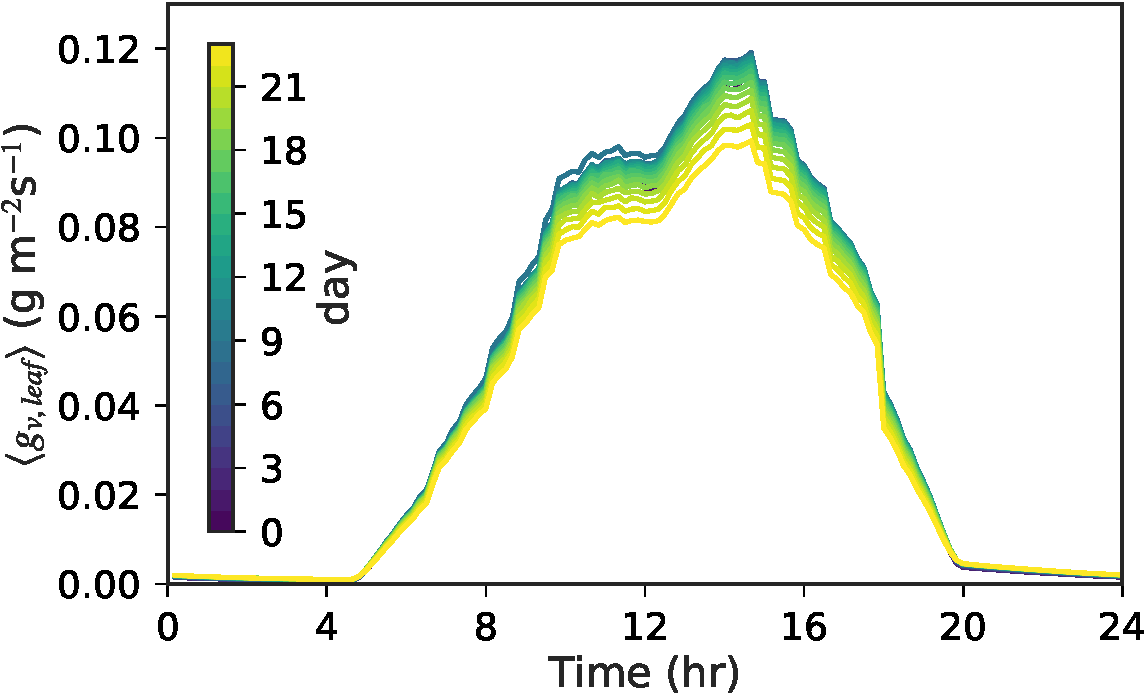
\includegraphics[width=0.8\textwidth]{\figdir/profile_gvleaf_collapsed-crop.pdf}
	\caption{profile gvleaf collapsed}
	\label{fig:profile_gvleaf_collapsed}
\end{figure}

\begin{figure}[t]
	\centering
	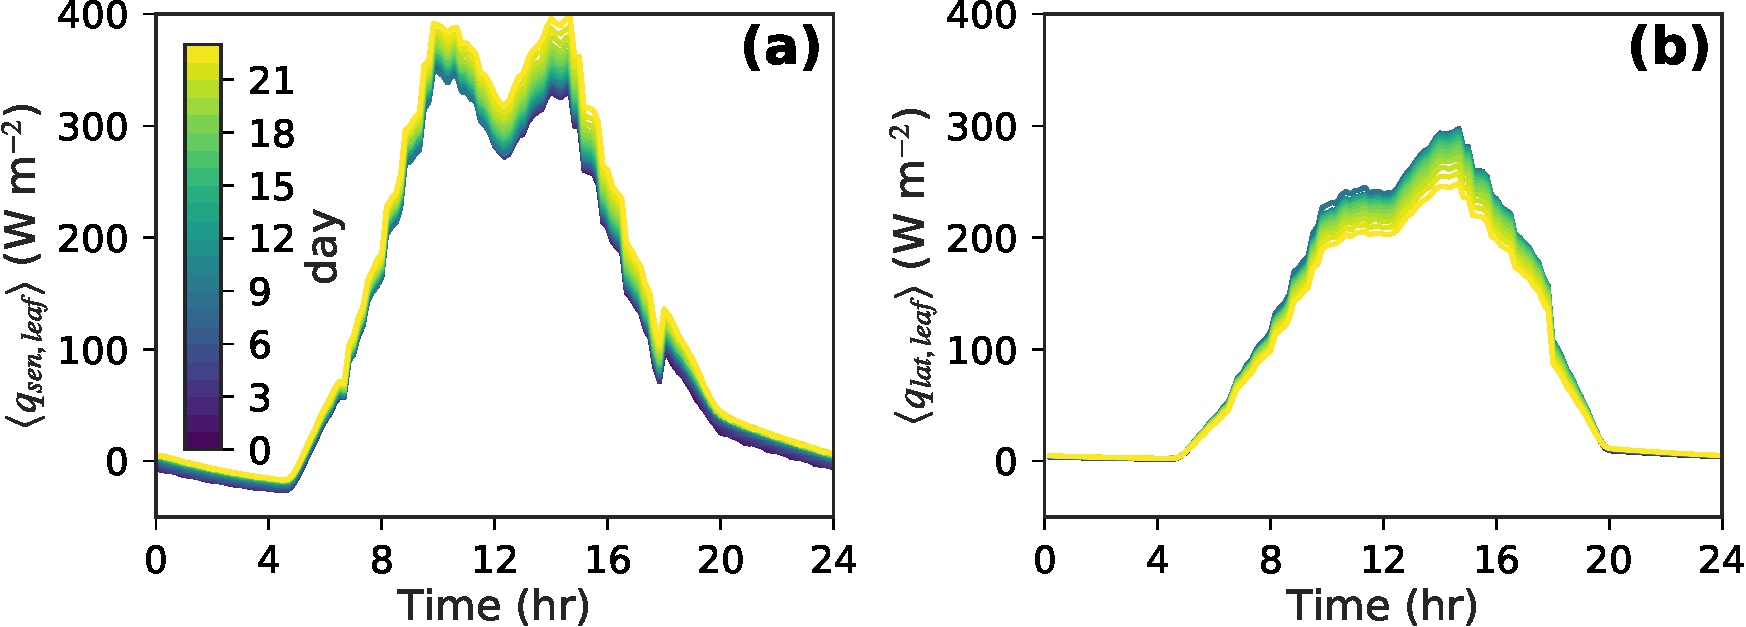
\includegraphics[width=\textwidth]{\figdir/energy_collapsed-crop.pdf}
	\caption{energy collapsed crop}
	\label{fig:energy_collapsed-crop}
\end{figure}


\subsection{Conclusion}

The present study investigates the influence of transpirative and tree-shade cooling on the microclimate of a street canyon. The study shows that both shading and transpiration have a direct influence on the temperatures measured in the street canyon. Furthermore, it is evident that tree-shade cooling is substantially larger than the transpirative cooling and, for the position of a pedestrian under the tree, the thermal comfort, measured through Universal Thermal Climate Index (UTCI), is only affected by the tree-shade cooling. In contrast, the transpirative cooling is seen to have negligible influence on the thermal comfort. Future studies will investigate the influence of environmental and vegetation properties on the impact of transpirative and tree-shade cooling. Additionally, the transpiration rate will be coupled with the soil moisture to determine the influence of root water availability on the impact of transpirative cooling.

The integrated model is used to study the influence of transpirative cooling and cooling due to shading of trees inside a street canyon. From this case study, both transpirative cooling and cooling through shading are seen to reduce the temperatures. Furthermore, the transpiration from the vegetation is seen to increase the humidity inside the street canyon. Although, this additional humidity is seen not to have a significant impact on pedestrian comfort, measured through universal thermal climate index (UTCI), as the comfort provided by the tree shading is substantially higher and counters the negative impacts of increased humidity. However, factors such as leaf area density (LAD), vegetation position, vegetation size, ambient conditions, etc. can have an influence on the outcome. Therefore, the influence of these parameters should be investigated to accurately estimate the impact of the vegetation in urban area.  

\section{Case study: Muensterhof}

\subsection{Simulation setup}

\subsection{Results and Discussion}

\subsection{Conclusion}
